\RequirePackage{fix-cm}
\documentclass[french]{article}
\usepackage[a4paper, total={6in, 10in}]{geometry}
\usepackage[T1]{fontenc}
\usepackage{babel}
\usepackage{hyperref}
\usepackage{enumitem}
\usepackage{tikz-qtree}
\usepackage{lscape}
\usepackage{graphicx}

\hypersetup{linkbordercolor = {1 1 1}}

\date{\today}

\title{Compte rendu projet Base de Données 2}
\author{\bsc{Billaud Maël} \and \bsc{Johan Quentin} \and \bsc{Ramé Tristan} \and \bsc{Goubon Valentin}} 
\date{Février 2022}

\begin{document}

\newlist{df}{enumerate}{2}
\setlist[df,1]{label=(\arabic*)}


\maketitle

\section{Première partie}
    \subsection*{Présentation Générale}
        Dans ce projet, l'objectif est de réaliser une base de données pas à pas. Pour ce faire, nous avons décidé de représenter la base de données d'un service de livraison de nourriture (Naofood, Deliveroo, ...). Nous avons donc défini ci-dessous un ensemble d'attributs permettant la gestion d'une telle organisation :\newline 
        U = \{\emph{nom\_resto, type\_cuisine, adr\_resto, tel\_resto, ouvert\_dimanche, note\_resto, nom\_client, prenom\_client, tel\_client, adr\_client, nom\_menu, prix\_menu, nom\_coursier, prenom\_coursier, note\_coursier, date\_course, mode\_deplacement}\}.
        

    \subsection*{Table générale}
        Pour des soucis de lisibilités, nous vous joignons notre table initiale, contenant tous les attributs ainsi qu'une dizaine de tuples, sous la forme d'un lien. Celui-ci vous mènera sur notre 
        \href{https://docs.google.com/spreadsheets/d/1HeSNFvLN3-yMfWHoYLVumzOeQpHXJHynqVBusbvl6EQ/edit?usp=sharing}{\underline{Google Sheet}}.
    
    
    
    \subsection*{Dépendances fonctionnelles}
        Vous trouverez ci-dessous les différentes dépendances fonctionnelles que nous avons trouvées pour notre table initiale.
        \begin{df}
            \item adr\_resto $\rightarrow$ nom\_resto, tel\_resto, ouvert\_dimanche
            \item nom\_client, prenom\_client $\rightarrow$ adr\_client, tel\_client
            \item nom\_menu $\rightarrow$ prix\_menu, nom\_resto
            \item nom\_coursier, prenom\_coursier $\rightarrow$  mode\_deplacement
            \item nom\_coursier, prenom\_coursier, date\_course, nom\_menu $\rightarrow$ note\_coursier, note\_resto
            \item nom\_resto $\rightarrow$ type\_cuisine
        \end{df}
        
        En calculant la clé à partir des DFs définies plus haut, on obtient : \newline
            clé = \{adr\_resto, nom\_client, prenom\_client, nom\_menu, nom\_coursier, prenom\_coursier, \newline date\_course\}
        \newpage
    \subsection*{Algorithmes de normalisation}
        \subsubsection *{Passage en 3FN, Algorithme de \bsc{Bernstein}}
            Pour appliquer l'algorithme suivant, on utilise la clé telle que définie plus haut. De manière évidente et en comparant avec les DFs, <R(U), DF> n'est pas en 3FN, on partitionne donc notre schéma en plusieurs ensembles :
            \begin{itemize}
                \item[$\bullet$] DF$_{1}$ = \{adr\_resto $\rightarrow$ nom\_resto, tel\_resto, ouvert\_dimanche\} \newline et U$_{1}$ = \{adr\_resto, nom\_resto, tel\_resto, ouvert\_dimanche\}
                
                \item[$\bullet$] DF$_{2}$ = \{nom\_client, prenom\_client $\rightarrow$ adr\_client, tel\_client\} \newline et U$_{2}$ = \{nom\_client, prenom\_client, adr\_client, tel\_client\}
                
                \item[$\bullet$] DF$_{3}$ = \{nom\_menu $\rightarrow$ prix\_menu, nom\_resto\} \newline et U$_{3}$ = \{nom\_menu, prix\_menu, nom\_resto\}
                
                \item[$\bullet$] DF$_{4}$ = \{nom\_coursier, prenom\_coursier $\rightarrow$  mode\_deplacement\} \newline et U$_{4}$ = \{nom\_coursier, prenom\_coursier, mode\_deplacement\}
                
                \item[$\bullet$] DF$_{5}$ = \{nom\_coursier, prenom\_coursier, date\_course, nom\_menu $\rightarrow$ note\_coursier, \newline note\_resto\} 
                \newline et U$_{5}$ = \{nom\_coursier, prenom\_coursier, date\_course, nom\_menu, note\_coursier, \newline note\_resto\}
                
                \item[$\bullet$] DF$_{6}$ = \{nom\_resto $\rightarrow$ type\_cuisine\} et U$_{6}$ = \{nom\_resto, type\_cuisine\}
            \end{itemize}
            
            \noindent
            On constate qu'aucun des schémas obtenus par le partitionnement ne contient de clé de R, on ajoute donc le schéma suivant :\newline
            DF$_{7}$ = \{\} et U$_{7}$ = \{adr\_resto, nom\_client, prenom\_client, nom\_menu, nom\_coursier, \newline prenom\_coursier, date\_course\}.\newline De plus, nous n'avons pas perdu d'information ni de dépendances fonctionnelles. Cette normalisation est donc \textbf{spi} et \textbf{spdf} où toutes les relations sont en \textbf{FN3}.
            
        \subsubsection *{Passage en FNBCK, Algorithme de Décomposition}
            L'algorithme que nous allons utiliser ci-dessous se base sur une décomposition récursive de Df ne contenant pas de clé à gauche. Celle-ci donne à chaque fois deux sous-relations qu'on décompose à nouveau si elles ne sont pas en FNBC.\newline Par soucis de lisibilité, nous allons désigner chacun des attributs par des lettres pour éviter que notre arbre de décomposition ne soit trop conséquent :
            \bigskip
            
 
            \begin{tabular}{lll}
                A = nom\_resto \\
                B = type\_cuisine \\
                C = adr\_resto \\
                D = tel\_resto \\
                E = ouvert\_dimanche \\
                F = note\_resto \\
                G = nom\_client \\
                H = prenom\_client \\
                I = tel\_client \\
                J = adr\_client \\
                K = nom\_menu \\
                L = prix\_menu \\
                M = nom\_coursier \\
                N = prenom\_coursier \\
                O = note\_coursier \\
                P = date\_course \\
                Q = mode\_deplacement \\
            \end{tabular}
            \hfill
            \begin{tabular}{ll}
                (1) & C $\rightarrow$ A,D,E \\
                (2) & G,H $\rightarrow$ I,J \\
                (3) & K $\rightarrow$ L,A \\
                (4) & M,N $\rightarrow$ Q \\
                (5) & M,N,P,K $\rightarrow$ O,F \\
                (6) & A $\rightarrow$ B \\
            \end{tabular}
            \bigskip
            
            La représentation de l'arbre de décomposition se trouve sur la page suivante :\newpage
                
            \begin{landscape}
                \thispagestyle{empty}
                \vspace*{\stretch{1}}
                \begin{tikzpicture}[sibling distance=20pt]
                    \tikzset{level distance=90pt, every tree node/.style={align=left, anchor=east}}
                    \Tree
                    [.{U = \{A, B, C, D, E, F, G, H, I, J, K, L, M, N, O, P, Q\} \\ DF = \{1, 2, 3, 4, 5, 6\}}
                        {U$_{1}$ = \{C, A, D, E\}\\ DF$_{1}$ = \{1\}} %U1
                        [.{U$_{2}$ = \{B, C, F, G, H, I, J, K, L, M, O, P, Q\}\\ DF$_{2}$ = \{2, 4, 5\}} %U2 
                            {U$_{21}$ = \{G, H, I, J\}\\ DF$_{21}$ = \{2\}} %U21 
                            [.{U$_{22}$ = \{B, C, F, G, H, K, L, M, N, O, P, Q\}\\ DF$_{22}$ = \{4, 5\}} %U22 
                                {U$_{221}$ = \{M, N, P, K, O, F\}\\ DF$_{221}$ = \{5\}} %U221 
                                [.{U$_{222}$ = \{B, C, G, H, K, L, M, N, P, Q\}\\ DF$_{222}$ = \{4\}} %U222 
                                    {U$_{2221}$ = \{M, N, Q\}\\ DF$_{2221}$ = \{4\}} %U2221 
                                    {U$_{2222}$ = \{B, C, G, H, K, L, M, N, P\}\\ DF$_{2222}$ = \{\}} %U2222 
                                ]
                            ]
                        ]
                    ]
                \end{tikzpicture}
                \vspace*{\stretch{1}}
            \end{landscape}
            \newpage
            
            Comme nous avons pu le voir avec le schéma ci-dessus, l'algorithme de normalisation par décomposition nous a donné 5 schémas:\bigskip
            \begin{enumerate}
                \item[$\bullet$] DF$_{1}$ = \{1\} et U$_{1}$ = \{adr\_resto, nom\_resto, tel\_resto, ouvert\_dimanche\}
                \item[$\bullet$] DF$_{21}$ = \{2\} et U$_{21}$ = \{nom\_client, prenom\_client, tel\_client, adr\_client\}
                \item[$\bullet$] DF$_{221}$ = \{5\} et U$_{221}$ = \{nom\_coursier, prenom\_coursier, date\_course, nom\_menu, \newline note\_coursier, note\_resto\}
                \item[$\bullet$] DF$_{2221}$ = \{4\} et U$_{2221}$ = \{nom\_coursier, prenom\_coursier, mode\_deplacement\}
                \item[$\bullet$] DF$_{2222}$ = \{\} et U$_{2222}$ = \{type\_cuisine, adr\_resto, nom\_client, prenom\_client, nom\_menu, prix\_menu, nom\_coursier, prenom\_coursier, date\_course\}\bigskip
            \end{enumerate}
            
            \noindent
            On peut remarquer que nous avons perdu 2 dépendances fonctionnelles au cours de la décomposition. Cette dernière est donc \textbf{uniquement spi} où toutes les relations sont en \textbf{FNBC}.
            
    \subsection*{Modèle Relationnel de la Base de Données}
        Grâces à nos algorithmes de normalisation, nous avons pu trouver deux schémas différents. Nous allons maintenant essayer de déterminer lequel des deux schémas obtenu nous donne le résultat le plus cohérents (sens des relations) et le plus qualitatif (formes normales).\newline
        D'un côté, un schémas trouvé par l'algorithme de Bernstein est en \textbf{3\up{eme} Forme Normale} alors que celui obtenu par l'algorithme de décomposition est en \textbf{Forme Normale de Boyce-Codd}. Ce dernier étant un plus grand gage de qualité que le 3FN, nous allons donc le préférer.\newline
        Cependant, lors que l'on regarde le shéma obtenu avec notre algorithme de décomposition, ce dernier n'est pas vraiment cohérent. En effet, l'attribut \emph{type de cuisine} est dans la relation qui contient les informations relatives à une commande alors qu'il serait plus logique qu'elle se rattache à celle correspondant au restaurant.\bigskip

        \begin{figure}[ht] %on ouvre l'environnement figure
            \centering
            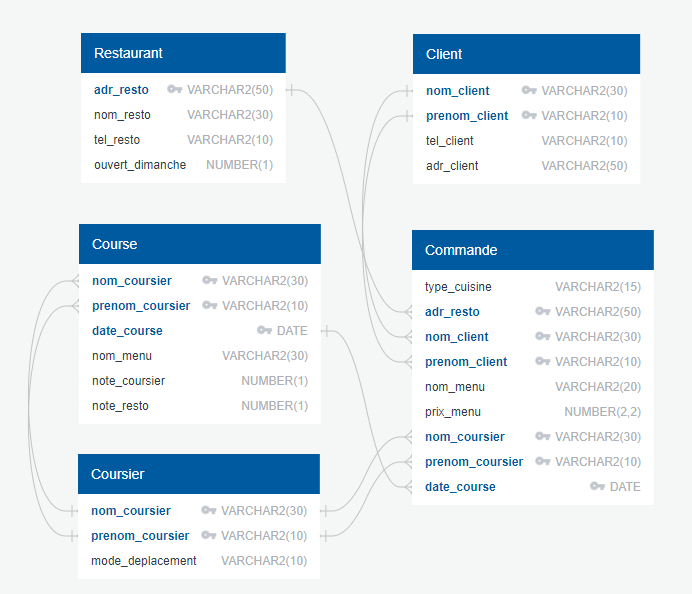
\includegraphics[scale = 0.7]{Image/modele_relationnel_1.png}
            \caption{Premier Modèle Relationnel de la Base de Données \emph{Service de Livraison de Nourriture}}
            \label{image_modele_relationnel_1}
        \end{figure}
        \newpage

        Nous allons donc essayer d'appliquer à nouveau l'agorithme de décomposition sur notre schéma initial mais avec des choix différents pour trouver un résultat plus satisfaisant. Dans cette décomposition, nous garderons les notations utilisées précédemment.\newline
        Après une seconde décomposition dont on ne détaillera pas l'arbre, nous obtenons les schémas suivants:\bigskip
        \begin{enumerate}
            \item[$\bullet$] DF$_{1}$ = \{6\} et U$_{1}$ = \{nom\_resto, type\_cuisine\}
            \item[$\bullet$] DF$_{21}$ = \{1\} et U$_{21}$ = \{adr\_resto, nom\_resto, tel\_resto, ouvert\_dimanche\}
            \item[$\bullet$] DF$_{221}$ = \{2\} et U$_{221}$ = \{nom\_client, prenom\_client, tel\_client, adr\_client\}
            \item[$\bullet$] DF$_{2221}$ = \{4\} et U$_{2221}$ = \{nom\_coursier, prenom\_coursier, mode\_deplacement\}
            \item[$\bullet$] DF$_{22221}$ = \{5\} et U$_{22221}$ = \{nom\_coursier, prenom\_coursier, date\_course, nom\_menu, \newline note\_coursier, note\_resto\} 
            \item[$\bullet$] DF$_{22222}$ = \{\} et U$_{22222}$ = \{adr\_resto, nom\_client, prenom\_client, nom\_menu, prix\_menu, nom\_coursier, prenom\_coursier, date\_course\}\bigskip
        \end{enumerate}
        Le résultat est presque le même, à ceci prêt qu'un nouveaux schéma apparait, séparant le \newline 
        \emph{type\_cuisine} de la table Commande. On obtient de ce fait le modèle relationnel suivant:\bigskip

        \begin{figure}[ht] %on ouvre l'environnement figure
            \centering
            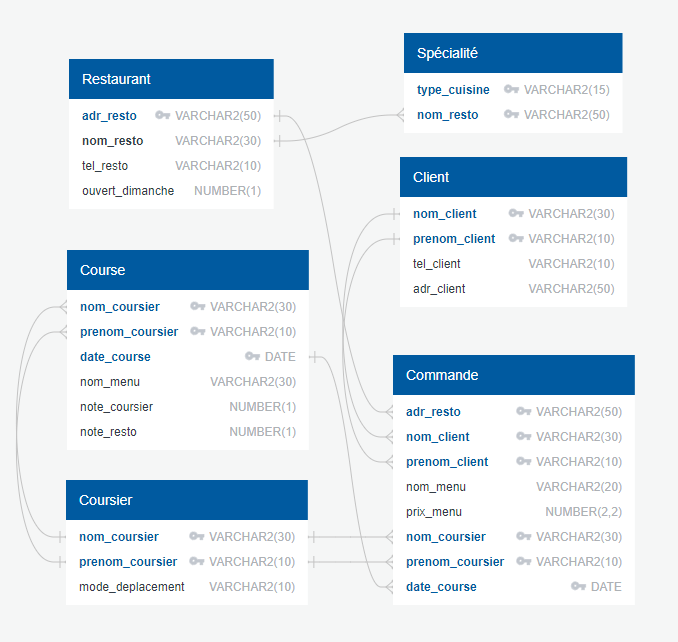
\includegraphics[scale = 0.7]{Image/modele_relationnel_2.png}
            \caption{Second Modèle Relationnel de la Base de Données \emph{Service de Livraison de Nourriture}}
            \label{image_modele_relationnel_2}
        \end{figure}
        \newpage

\section{Seconde partie}
        \subsection*{Création des tables}


        \subsubsection*{Creation d'indexe}
        Nous avons choisi de créer un indexe sur les attributs \textit{mon\_menu} et textit{prix\_menu} de la table Commande. Ce choix nous semble jusdicieux car cette table sera la plus utilisé avec la table Courses (à chaque nouvelle commande, ce qui est le plus fréquent, un nouveau tuple de cette table est créé). De plus, elle ne sera pas modifiée. Lorsqu'une commande est effectuée, on veut soit regarder les informations qu'elle contient, soit la supprimer si elle est erronnée mais une fois la commande passée, on ne peut pas la modifier. 
            
        \subsubsection*{Création de séquence}
            Une séquence est un objet de Base de Donnée qui permet de générer des numéros séquentiels (qui peuvent notamment être utilisés pour créer des clés primaires uniques de manière automatique). Dans notre base de donné, nous n'avons pas besoin d'identifiants dans nos tables. Nous allons alors créer une séquence spécifique à notre table \textit{Commande} qui nous permettra de compter le nombre de commande qui ont été passées depuis la création de notre BD.

        \subsubsection*{Insertion des Tuples}
            Nous avons repris la tuples que nous avions fait au tout début de notre projet que vous pouvez retourver sur notre \href{https://docs.google.com/spreadsheets/d/1HeSNFvLN3-yMfWHoYLVumzOeQpHXJHynqVBusbvl6EQ/edit?usp=sharing}{\underline{Google Sheet}}. Nous les avons simplement adaptés pour qu'ils s'insèrent dans les tables créer précédemment.\newline
            Nous avons cependant rencontré un problème concernant notre attribut \textit{date\_course}. Il correspond donc à la date de la courses mais aussi à son heure (pour qu'un même coursier puisse faire plusieurs courses en une seule journée). Cependant, malgré ce qu'on peut trouver dans la document d'Oracle, le type DATETIME n'est pas reconnu pour notre base de données. Nous avons donc du recourrir à la fonction to\_date pour pouvoir garder le type DATE tout en évitant les erreurs dues aux contraintes d'intégrités. Cependant, l'affichage dans sqlplus ne prend pas en compte les heures de notre attribut \textit{date\_course}. 

        \subsection*{Utilisation du PLSQL et des Vues}

            \subsubsection*{Triggers}
                BLABLABLABLABLABLABLABLA
            
            \subsubsection*{Fonctions et Procédures}
            BLABLABLABLABLABLABLABLA
            
            \subsubsection*{Vues}
            BLABLABLABLABLABLABLABLA

        \subsection*{Gestion des droits}
            \subsubsection*{Création des rôles}
                Pour la création des rôles, nous avons essayer de nous rapprocher au plus de ce qui, selons nous, était l'organisation d'un vrai service de livraison de nourriture (simplifié bien entendu).
                Nous avons donc créé des rôles pour : 
                \begin{itemize}
                    \item un administrateur de la Base de Donnée (\textit{DB\_admin})
                    \item un directeur du service (\textit{CEO})
                    \item les coursiers (\textit{Coursier})
                    \item les restaurants (\textit{Restaurateur})
                    \item les clients (\textit{Client})
                \end{itemize}
            
            \subsubsection*{Attribution des droits aux rôles}
                Concernant l'attribution des droits aux rôles, nous avons réfléchis de la manière suivante : Qu'est ce que chaque acteur de notre Bases de Données doit pouvoir faire et ne doit pas pouvoir faire ?

                \begin{description}
                    \item[$\bullet$]Le Client\newline
                     Il doit pouvoir regarder les différents restaurants ainsi que leurs type de nourriture pour pouvoir choisir sa commande. Il doit également pouvoir s'enregistrer en tant que client (mais aussi modifier son compte )et effectuer une commande (ou la modifier si il veut changer de menu). Par la suite, nous considèrerons que des qu'un rôle permetra d'insérer des tuples dans une table, il permetra également de modifier les tuples insérés.

                    \item[$\bullet$]Le Restaurateur\newline
                     Il doit pouvoir avoir accès au informations concernant les commande pour pouvoir les effectuer. Mais aussi s'enregistrer en tant que restaurant et renseigner sa spécialité.

                    \item[$\bullet$]Le Coursier\newline
                     Il doit pouvoir vérifier les données concerannt sa commande, mais aussi celles du Client pour connaître son adresse ou encore son numéro de téléphone. Il doit également pouvoir s'enregistrer en tant que coursier.

                    \item[$\bullet$]Le CEO\newline
                     Il doit pour avoir accès à toute les informations de la base de données mais aussi pouvoir ajouter ou modifier des données en fonction des besoins de son entreprise. 

                    \item[$\bullet$]L'administrateur de la Base de Données\newline
                     Ce dernier doit pourvoir agencer pleinement la base de données. Nous allons donc lui donner tous les privilèges.  
                \end{description}

                Ces deux derniers rôle représentent un potentiel danger pour la base de donnée de part leur grand permissibilité. Nous avons donc décider de les protéger par des mots de passe.\newline
                Comme chacun des rôles est très spécifique, nous n'avons cependant pas pu mettre en place la notion d'héritage.

            \subsubsection*{Attribution des rôles aux utilisateurs}
                Pour l'attribution des rôles aux utilisateurs, chaque memebre du groupe s'est vu assigner un rôle différent. Comme nous sommes peu comparé au nombre d'utilisateurs que pourrait acceuillir une véritable base de donnée d'un service de livraiso de nourriture, nous n'avons pas pu former de groupe d'utilisateurs.
\end{document}